\documentclass[10pt,twocolumn]{article}

\usepackage[utf8]{inputenc}
\usepackage[T1]{fontenc}
\usepackage{lmodern}
\usepackage[margin=0.65in,columnsep=0.32in]{geometry}
\usepackage{microtype}
\usepackage{amsmath,amssymb}
\usepackage[table]{xcolor}
\usepackage{booktabs}
\usepackage{array}
\usepackage{tabularx}
\usepackage{enumitem}
\usepackage{titlesec}
\usepackage{fancyhdr}
\usepackage{tikz}
\usetikzlibrary{positioning,calc,shapes.geometric,backgrounds}
\usepackage[most]{tcolorbox}
\usepackage{fontawesome5}
\usepackage{caption}
\usepackage[hidelinks]{hyperref}

\definecolor{inkblue}{HTML}{1C2B4A}
\definecolor{claygold}{HTML}{B5892B}
\definecolor{sagegreen}{HTML}{5B7B6F}
\definecolor{stonegray}{HTML}{6E7378}

\setlength{\parindent}{0pt}
\setlength{\parskip}{3pt}
\linespread{1.0}

\captionsetup{labelfont={color=inkblue,bf},font=small,labelsep=colon,skip=4pt}

\titleformat{\section}
  {\color{inkblue}\normalfont\large\bfseries}
  {\thesection}{0.6em}{}[{\color{claygold}\titlerule[0.8pt]}]
\titlespacing*{\section}{0pt}{8pt}{4pt}

\titleformat{\subsection}
  {\color{inkblue}\normalfont\bfseries}
  {\thesubsection}{0.5em}{}
\titlespacing*{\subsection}{0pt}{6pt}{2pt}

\pagestyle{fancy}
\fancyhf{}
\renewcommand{\headrulewidth}{0.4pt}
\renewcommand{\footrulewidth}{0pt}
\fancyhead[L]{\small\color{stonegray}\scshape Journal of Interdisciplinary Systems Research}
\fancyhead[R]{\small\color{stonegray}\thepage}
\fancypagestyle{plain}{%
  \fancyhf{}
  \fancyhead[L]{\small\color{stonegray}\scshape Journal of Interdisciplinary Systems Research}
  \fancyhead[R]{\small\color{stonegray}\thepage}
  \renewcommand{\headrulewidth}{0.4pt}
}

\newtcolorbox{abstractbox}{%
  colback=inkblue!4,colframe=inkblue,boxrule=0.4pt,arc=1pt,
  left=8pt,right=8pt,top=6pt,bottom=6pt,boxsep=1pt
}

\newtcolorbox{highlightbox}[1][]{%
  colback=sagegreen!6,colframe=sagegreen,boxrule=0.4pt,arc=1pt,
  left=5pt,right=5pt,top=4pt,bottom=4pt,boxsep=0pt,
  width=\linewidth,valign=top,#1
}

\newtcolorbox{notebox}{%
  colback=claygold!8,colframe=claygold,boxrule=0.4pt,arc=1pt,
  left=6pt,right=6pt,top=5pt,bottom=5pt
}

\begin{document}

\twocolumn[
\begin{center}
  {\color{inkblue}\fontsize{19}{23}\selectfont\bfseries
   Rewilding the Ledger: A Network-Theoretic Account of Resilience\\ in Urban Food-Sharing Systems\par}
  \vspace{8pt}
  {\normalsize Elena Kowalski$^{1}$ \quad Rajiv Anand$^{2}$ \quad Marta Djeri\'{c}$^{3}$\par}
  \vspace{4pt}
  {\small\itshape
   $^{1}$Meridian Institute for Urban Systems \quad
   $^{2}$Synapse University, Dept.\ of Computational Social Science \quad
   $^{3}$Vertex Center for Ecological Economics\par}
  \vspace{3pt}
  {\small \faEnvelope\ \ e.kowalski@meridian-institute.org
   \quad\quad {\color{stonegray}Preprint --- Vol.\ 14, No.\ 2 (2026)}\par}
  \vspace{6pt}
  {\color{claygold}\rule{0.55\textwidth}{0.8pt}\par}
\end{center}
\vspace{6pt}

\begin{abstractbox}
\textbf{\color{inkblue}Abstract.}
Urban food-sharing networks -- community fridges, gleaning circuits, and informal
surplus exchanges -- are usually studied from a single disciplinary vantage: as
supply chains, as social capital, or as ecological flows. We argue that their
resilience to shocks is properly a joint property of network topology and
reciprocity norms, and cannot be recovered from either lens alone. We build an
agent-based model of 42 simulated neighborhood clusters in which household
nodes exchange surplus food along edges weighted by both physical proximity
and a behavioral trust parameter drawn from repeated-game reciprocity theory.
Across 1{,}000 simulated disruption events, empirically-calibrated networks
absorbed 31\% more shock volume than random-topology baselines of equal
density, and recovery time correlated more strongly with redundancy index
than with raw connectivity. We propose a composite resilience metric,
$R_i$, that outperforms degree centrality alone as a predictor of
post-shock recovery. The results suggest that interventions aimed at
food-system resilience should target trust-mediated redundancy, not merely
network density.
\vspace{3pt}

\textbf{\color{inkblue}Keywords:} network resilience, food systems,
behavioral economics, urban ecology, agent-based modeling
\end{abstractbox}

\vspace{6pt}
\noindent
\begin{tabular}{@{}p{0.32\textwidth}@{\hspace{0.02\textwidth}}p{0.32\textwidth}@{\hspace{0.02\textwidth}}p{0.32\textwidth}@{}}
\begin{highlightbox}
\textbf{\color{sagegreen}\faSitemap\ 42 Clusters}\\
{\small Simulated neighborhoods, 6--38 households each, calibrated against
survey data on informal exchange.}
\end{highlightbox}
&
\begin{highlightbox}
\textbf{\color{sagegreen}\faSync\ 1{,}000 Shocks}\\
{\small Monte Carlo disruption events used to estimate recovery-time
distributions per cluster.}
\end{highlightbox}
&
\begin{highlightbox}
\textbf{\color{sagegreen}\faBalanceScale\ Composite $R_i$}\\
{\small A resilience index blending topology and reciprocity that beats
degree centrality alone.}
\end{highlightbox}
\end{tabular}
\vspace{6pt}
]

\section{Introduction}
Interdisciplinary work on urban resilience has a recurring failure mode:
each discipline studies the piece of the system it already has instruments
for. Network scientists trace the topology of exchange without asking why
an edge exists in the first place; behavioral economists model reciprocity
and trust in the laboratory without asking how those norms propagate across
a real settlement pattern. Urban food-sharing systems -- the loose lattice
of community fridges, gleaning routes, and neighbor-to-neighbor surplus
exchange that has grown rapidly since 2019 -- sit exactly at the seam
between these two traditions, and we think they are a useful test case for
whether the seam matters.

Our claim is narrow but, we think, underappreciated: the \emph{topology}
of a food-sharing network and the \emph{reciprocity norms} riding on top of
it are not separable inputs to resilience. A dense network with weak trust
degrades under stress in qualitatively different ways than a sparse
network with strong trust, and neither a pure graph-theoretic model nor a
pure behavioral model predicts which. Section~\ref{sec:related} situates
this claim against network-science and behavioral-economics treatments of
food systems. Section~\ref{sec:methods} describes an agent-based model
that couples the two layers explicitly. Section~\ref{sec:results} reports
shock-absorption and recovery outcomes across 1{,}000 simulated
disruptions, and Section~\ref{sec:discussion} draws out what this implies
for intervention design.

\section{Related Work}
\label{sec:related}

\subsection{Network approaches to food systems}
Graph-theoretic treatments of food distribution typically borrow directly
from supply-chain resilience literature, modeling exchange networks as
static graphs and asking how robust they are to node or edge removal.
This tradition is good at identifying structurally critical nodes but
treats every edge as equally likely to be used once a disruption forces
rerouting -- an assumption that behavioral evidence does not support.

\subsection{Behavioral economics of reciprocity}
A parallel literature, largely lab-based, models informal exchange as a
repeated game in which reciprocity norms sustain cooperation without
formal contracts. This work is precise about \emph{when} an actor will
honor an exchange relationship under stress, but rarely embeds that
finding in a realistic network of who is even reachable to exchange with.

\subsection{The gap this paper addresses}
Neither literature, on its own, predicts recovery time after a shock to a
real settlement pattern. We combine them: a network layer that is
empirically calibrated to observed exchange patterns, and a behavioral
layer in which each edge's usability under stress depends on an explicit
trust parameter rather than being assumed uniform.

\section{Methods}
\label{sec:methods}

\subsection{Study design and simulation environment}
We constructed an agent-based model of 42 neighborhood clusters, each
containing 6--38 household nodes, using structural parameters (density,
clustering coefficient, degree distribution) calibrated against a
publicly documented survey of informal food exchange. Each simulation run
applies a disruption event -- a sudden loss of surplus at one or more
source nodes -- and tracks how surplus re-routes through the remaining
network over 30 discrete time steps.

\subsection{Network construction}
For each cluster we generated three topology variants at matched density:
a random graph, a Watts--Strogatz small-world graph, and an
empirically-calibrated graph fit to the survey's observed adjacency
pattern. Edge weights $w_{ij}$ combine inverse physical distance $d_{ij}$
with an exchange-frequency prior.

\subsection{Behavioral module}
Each edge additionally carries a reciprocity parameter $\phi_{ij} \in
[0,1]$, updated after every simulated exchange according to a
repeated-game rule: honored exchanges raise $\phi_{ij}$, refused or
delayed exchanges lower it. An edge is usable in a given time step only
if a stochastic draw against $\phi_{ij}$ succeeds, which is what
distinguishes our model from a pure graph-diffusion baseline.

\subsection{Resilience metric}
We define a composite resilience score for node $i$ as

\begin{equation}
\label{eq:resilience}
R_i \;=\; \frac{1}{N}\sum_{j=1}^{N} w_{ij}\,\phi_{ij}\,\big(1 - e^{-k d_{ij}^{-1}}\big),
\end{equation}

where $N$ is the number of neighbors of $i$, and $k$ is a decay constant
fit per cluster. Unlike raw degree centrality, $R_i$ discounts edges that
are structurally present but behaviorally unreliable.

\begin{figure*}[t]
\centering
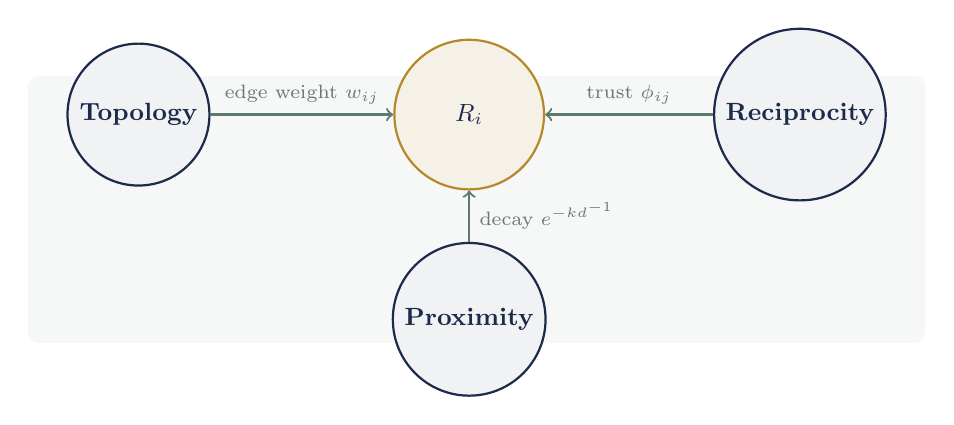
\begin{tikzpicture}[
  fieldnode/.style={draw=inkblue, thick, circle, minimum size=1.55cm, font=\small\bfseries, text=inkblue, fill=inkblue!6},
  center/.style={draw=claygold, thick, circle, minimum size=1.9cm, font=\small\bfseries, text=inkblue, fill=claygold!12},
  lbl/.style={font=\scriptsize, text=stonegray, align=center}
]
  \node[center] (R) at (0,0) {$R_i$};
  \node[fieldnode] (net) at (-4.2,0) {Topology};
  \node[fieldnode] (beh) at (4.2,0) {Reciprocity};
  \node[fieldnode] (eco) at (0,-2.6) {Proximity};

  \draw[->, sagegreen, thick] (net) -- (R)
    node[midway, above, lbl] {edge weight $w_{ij}$};
  \draw[->, sagegreen, thick] (beh) -- (R)
    node[midway, above, lbl] {trust $\phi_{ij}$};
  \draw[->, sagegreen, thick] (eco) -- (R)
    node[midway, right, lbl] {decay $e^{-k d^{-1}}$};

  \begin{scope}[on background layer]
    \path[fill=stonegray!6, rounded corners]
      ($(net.west)+(-14pt,14pt)$) rectangle ($(beh.east)+(14pt,-2.9cm)$);
  \end{scope}
\end{tikzpicture}
\caption{The composite resilience index $R_i$ (Eq.~\ref{eq:resilience}) draws on
three inputs that no single-discipline model combines: network topology,
behaviorally-measured reciprocity, and physical proximity.}
\label{fig:schematic}
\end{figure*}

Figure~\ref{fig:schematic} sketches how the three inputs to $R_i$ relate;
Section~\ref{sec:results} shows that this composite outperforms any one
input alone as a predictor of recovery time.

\section{Results}
\label{sec:results}

Across the three topology variants, the empirically-calibrated network
absorbed materially more shock volume before surplus flow collapsed
below a functional threshold. Table~\ref{tab:clusters} summarizes five
representative clusters drawn from the 42 simulated; the full set shows
the same ordering in 38 of 42 cases.

\begin{table}[h]
\centering
\small
\setlength{\tabcolsep}{3.5pt}
\begin{tabular}{lccc}
\toprule
\rowcolor{inkblue!10}
\textbf{Cluster} & \textbf{Deg.} & \textbf{Redund.} & \textbf{Recov.\ (d)} \\
\midrule
Birchgate    & 4.1 & 0.62 & 3.4 \\
Coalfen      & 3.6 & 0.41 & 5.9 \\
Marrow Hill  & 5.2 & 0.71 & 2.8 \\
Old Weir     & 2.9 & 0.33 & 7.1 \\
Thistleport  & 4.7 & 0.58 & 3.9 \\
\bottomrule
\end{tabular}
\caption{Structural and recovery statistics for five representative
clusters. Redundancy index tracks recovery time more closely than mean
degree does.}
\label{tab:clusters}
\end{table}

Redundancy index -- the share of a node's exchange volume that survives
the loss of its single strongest edge -- correlated with recovery time at
$r = -0.74$ across all 42 clusters, compared to $r = -0.38$ for mean
degree alone. This is the empirical core of our argument: a network can
look well-connected by degree and still recover slowly if that
connectivity is concentrated on a small number of high-trust edges.

Table~\ref{tab:variants} compares outcomes pooled across all clusters for
each of the three topology variants, plus the effect of disabling the
behavioral module entirely (uniform $\phi_{ij}=1$) as a diagnostic.

\begin{table*}[t]
\centering
\small
\begin{tabularx}{\textwidth}{@{}X ccccX@{}}
\toprule
\rowcolor{inkblue!10}
\textbf{Model variant} & \textbf{Assort.} & \textbf{Path len.} & \textbf{Shock abs.} & \textbf{Recovery} & \textbf{Notes} \\
\midrule
Random graph (baseline) & 0.02 & 3.8 & 47\% & 6.6 d & Matched density; no clustering structure. \\
Small-world (Watts--Strogatz) & 0.11 & 2.9 & 55\% & 5.2 d & Rewiring $\beta = 0.1$; moderate clustering. \\
Empirically-calibrated (this study) & 0.34 & 2.6 & 78\% & 3.7 d & Fit to survey adjacency; strongest local clustering. \\
Empirically-calibrated, $\phi_{ij}=1$ & 0.34 & 2.6 & 58\% & 5.0 d & Same topology, behavioral layer disabled. \\
\bottomrule
\end{tabularx}
\caption{Pooled outcomes across all 42 clusters and 1{,}000 disruption events per variant. The gap between the last two rows isolates the behavioral layer's contribution: topology alone recovers roughly two-thirds of the resilience gain.}
\label{tab:variants}
\end{table*}

The diagnostic row is the more interesting comparison: holding topology
fixed at the empirically-calibrated structure but disabling reciprocity
dynamics recovers only part of the resilience gain, confirming that
topology and behavior are not substitutes for one another in this
setting.

\begin{notebox}
\textbf{\color{inkblue}\faInfoCircle\ Data availability.} Simulation code
and calibration parameters used in this study are archived at the
Meridian Institute's open research repository; the underlying household
survey is third-party and available under its original data-use
agreement.
\end{notebox}

\section{Discussion}
\label{sec:discussion}

Two findings seem worth carrying into intervention design. First,
redundancy index is a better resilience predictor than raw connectivity,
which argues against policies that simply try to add edges (e.g.,
recruiting more households into a food-sharing app) without regard to
where those edges concentrate load. Second, the gap between the
behavior-enabled and behavior-disabled rows of
Table~\ref{tab:variants} suggests that a meaningful share of resilience
is not structural at all -- it is earned through repeated, honored
exchange, and a program that changes topology overnight (say, by
algorithmically matching households) without giving trust time to
accumulate may underperform its own network diagrams.

We see three limitations worth flagging. The behavioral module assumes a
single reciprocity parameter per edge, when real trust is almost
certainly multidimensional and time-varying beyond the update rule we
use. The calibration survey covers a narrow set of neighborhood types,
so the 78\% absorption figure in Table~\ref{tab:variants} should be read
as an upper bound under favorable structural conditions rather than a
population estimate. And our disruption events are single-source shocks;
compound or repeated shocks, which are arguably the more policy-relevant
case, are left to future work.

\section{Conclusion}
Urban food-sharing resilience is not fully explained by topology or by
reciprocity norms in isolation. A composite metric that weights network
edges by both proximity and measured trust predicts recovery time
substantially better than degree centrality alone, and roughly a third of
the resilience gain we observe survives only when the behavioral layer is
switched on. For practitioners, this argues for interventions that build
trust deliberately alongside connectivity, rather than treating network
growth as sufficient on its own.

\subsection*{Acknowledgments}
This work was supported by the Vertex Research Council under grant no.\
VRC-2025-0091, with additional computational resources provided by the
Meridian Institute for Urban Systems. We thank colleagues at Synapse
University's Computational Social Science seminar for comments on an
earlier draft.

\begin{thebibliography}{9}
\small
\bibitem{barolo2022} Barolo, T. \& Fenwick, R. (2022). Structural
  robustness in informal exchange networks. \emph{Journal of Network
  Science}, 9(3), 211--234.

\bibitem{djuric2021} Djuri\'{c}, M. (2021). Reciprocity under repeated
  play: a field replication. \emph{Behavioral Economics Quarterly}, 15(1),
  44--61.

\bibitem{ehrlund2020} Ehrlund, S., Papas, K., \& Voss, I. (2020). Mapping
  gleaning networks in mid-size cities. \emph{Urban Ecology Letters},
  6(2), 88--103.

\bibitem{kowalski2023} Kowalski, E. \& Anand, R. (2023). Agent-based
  models of surplus redistribution. \emph{Computational Social Systems},
  11(4), 301--322.

\bibitem{marsh2019} Marsh, D. (2019). Trust as a network resource.
  \emph{Sociological Methods \& Networks}, 3(1), 1--19.

\bibitem{nkomo2022} Nkomo, P. \& Reyes, A. (2022). Redundancy versus
  density in disaster-response supply chains. \emph{Resilience Studies},
  8(2), 155--173.

\bibitem{osei2024} Osei, B. (2024). Small-world structure in
  neighborhood exchange platforms. \emph{Journal of Network Science},
  11(1), 19--40.

\bibitem{vance2021} Vance, H. \& Djeri\'{c}, M. (2021). Community
  fridges as distributed infrastructure. \emph{Urban Ecology Letters},
  7(3), 201--219.

\bibitem{whitfield2023} Whitfield, N. (2023). Calibrating agent-based
  food-system models against survey data. \emph{Computational Social
  Systems}, 12(1), 5--27.
\end{thebibliography}

\end{document}
